\chapter{Introduction}
\vspace*{0.5cm}
\setcounter{page}{1}
\pagenumbering{arabic}

%Since the start of 2020 \textit{Sars-COVID19} has initiated a world-wide pandemic. In an attempt to slow down the fast and uncontrollable spread of this disease various prevention and diagnosis methods have been developed. In this work, out of all these various methods, the attention is going to be put on the possible developement diagnostic methods related to medical images, be they automatic or semi-automatic, to be intended either as Clinical Decision Support Systems (CDSS) or as a quick evaluation to completely avoid human analysis.
%In this light this first introductory chapter is going to start from a basic theoretical overview of the necessary core concepts that will be needed throughout this whole work such as definition of an image and imaging methods, with particular attention to those used in the medical field. This will be followed by an introduction to Artificial Intelligence (AI) and some Machine Learning techniques. Finally some of the concepts from the two previous topics will be treated jointly under the discipline of radiomics, which will be defined and explored as necessary.

Nowadays everybody knows of  \textit{Sars-COVID19} which, since the start of 2020, has made necessary a few world-wide quarantines forcing everybody in self-isolation. It is also well known that, among the main complications and features of this virus, symptoms gravity as well as the rate of deterioration of the conditions are some of the most relevant and problematic. In some cases asymptomatic or near to asymptomatic people may, in the span of a week, get to conditions that require hospital admission. This peculiarity is also what heavily complicates the triage process, since trying to predict with some degree of accuracy the prognosis of the patient at admission is a thoroughly complex task. In this thesis the aim will be to use data, specifically including data that cannot be easily interpreted by humans, to try various methods to predict a couple of clinical outcomes, namely the death of the patient or the admission in the Intensive Care Unit (ICU), while assessing their performance. These analyses will be carried out on a dataset of 434 patients with different variables associated to every person. A part of the variables, which will be called clinical and radiological, are defined by humans and are generally discrete in nature but mostly boolean. The most part of the available variables, however, will be image-derived following the approaches used in the field of radiomics. While the utility of clinical variables, such as age, obesity and history of smoking, is very straightforward it's interesting and helpful to understand the basis behind the utility of radiomic and radiological features.

Generally speaking it's clear that images have the ability to convey a slew of useful images, this is expecially true in the medical field where digital images are used to inspect also the internal state of the patient giving far more detailed information than that obtainable by visual inspection at the hand of medical professionals. Among the ways in which \textit{Sars-COVID19} can manifest himself the one that is most relevant to the scopes of this thesis pneumonia and the complications that stem from it. Some of these complications, which are not specific of \textit{Sars-COVID19} but can happen in any pneumonia case, display very peculiar patterns when visualizing the lungs through CT exams.

These patterns are due to the pulmonary response to inflammation which may lead to thickening of the bronchial and alveolar structures up to pleural effusions and collapsed lungs. Without going too much in clinical detail what is of interest is how these condition manifest themselves in the CT exams:

\todo[inline]{li sposterei in capitoli successivi}
\begin{enumerate}
        \item \textbf{Ground Glass Opacity(GGO)}:\newline Small diffused changes in density of the lung structure cause a hazy look in the affected region. This complicates the individuation of pulmonary vessels.
			\begin{figure}[htbp]
				\centering
				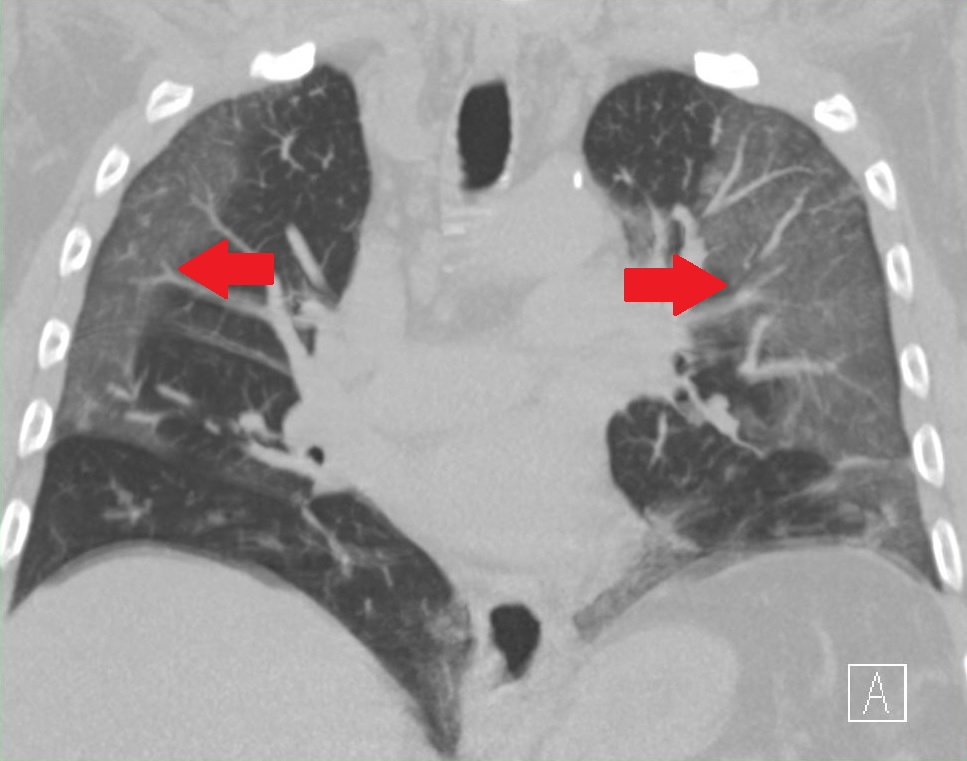
\includegraphics[width=0.66\linewidth]{GGO.jpg}
				\caption{Example of GGO\label{GGOImage}}
			\end{figure}
        \item \textbf{Lung Consolidations}:\newline Heavier damage reflects in whiter spots in the lung as the surface more closely resembles outside tissue instead of normal air. The consolidation refer to presence of fluid, cells or tissue in the alveolar spaces
        \item \textbf{Crazy paving}:\newline When GGOs are superimposed with inter-lobular and intra-lobular septal thickening.
			\begin{figure}[htbp]
				\centering
				\subfloat[][a]{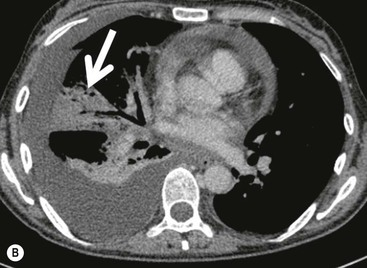
\includegraphics[width=0.35\linewidth]{CollapsedLung.jpg}}
				\subfloat[][a]{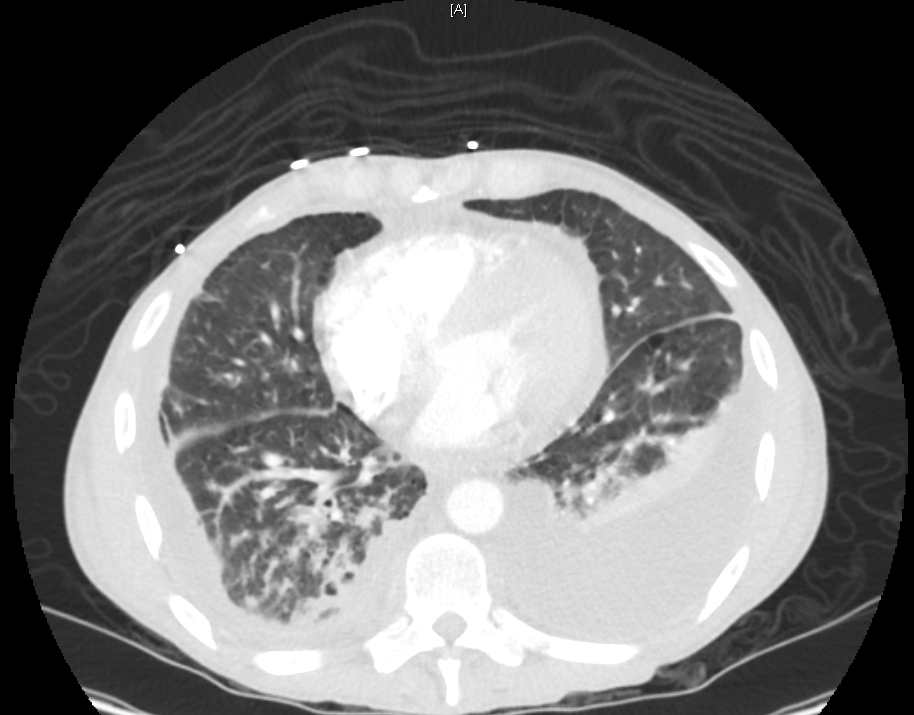
\includegraphics[width=0.33\linewidth]{PleuralEffusion.png}}
				\caption{Differences between a collapsed lung (a) and pleural effusion(b)}
			\end{figure}
	\item \textbf{Collapsed Lungs and Pleural Effusion}:\newline Both of these manifest themself as regions of the lungs that take the same coloring as that of tissue outside the lung. The main difference between the two is that collapsed lungs are somewhat rigid structures, they can occur in singular lobes of the lung and stay where they occur. Pleural effusions, however, are actually fluid being located in the lung instead of air. As such these lesions usually are located 'at the bottom' of the lung in which they happen and migrate to the lowest part of the lung according to the position of the patient.
\end{enumerate}

Having these manifestation it's clear that they are mainly textural and intensity-like changes in the normal appearance of the lungs. However, whereas these properties can be easily described in a qualitative and subjective way, it's rather complex to describe them in a quantitative and objective way. The field of radiomics, when coupled with digital images and preprocessing steps which must include image segmentation, is exactly what undertakes this daunting task. Radiomics comes from the the combination of radiology and the suffix \textit{-omics}, which is characteristic of high-throughput methods that aim to generate a large number of numbers, called biomarkers or features, as such it uses very precise and strict mathematical definitons to quantify in various ways either shape, textural or intensity based properties of the radiological image under analysis.

Given the large numerosity of the features produced by radiomics it's necessary to analyze these kinds of data with methods that rely on Machine Learning and their ability to address high-dimensional problems, be it in a supervised or unsupervised way, in a rather fast and accurate way.

Starting from these premises this thesis will be divided in a few chapters and sections. The first step will be taken by providing the general theoretical background regarding the aforementioned topics and techniques, this will be followed by a desscription of the data in use as well as a presentation of the analysis methods and resources used. Finally the results of the methods described will be presented and from them a set of concluding remarks will be set forth.

\section{Medical Images}
In this section the objective is to simply provide a set of basic definitions pertaining to images as well as a general introduction to the methods used to create said images. Firstly images are a means of representing in a visual way a physical object or set thereof, when talking about images it's common to refer specifically to digital images.

\begin{definition}[Digital Image]
A numerical representation of an object; more specifically an ordered array of values representing the amount of radiation emitted (or reflected) by the object itself. The values of the array are associated to the intensity of the radiation coming from the physical object; to represent the image these values need to be associated to a scale and then placed on a discrete 2D grid.
To store these intensities the physical image is divided into regular rectangular spacings, each of which is called pixel\footnote{The term pixel seems to originate from a shortening of the expression Picture's (pics=pix) Element(el). The same hold for voxel which stands for Volume Element}, to form a 2D grid; inside every spacing is then stored a number (or set thereof) which measures the intensity of light, or color, coming from the physical space corresponding to that grid-spacing.
The term digital refers to the discretization process that inherently happens in storage of the values, called pixel values, as well as in arranging them within the grid. It's possible to generalize from 2D images to 3D volumes, simply by stacking images of the same object obtained at different depths. In this context, the term pixel is substituted by voxel, however since they are used interchangeably in literature they will, from now on, be considered equivalent.
\end{definition}

Generally pixel values stored as integers p$\in$ [0,2$^{n}$-1] with p,n$\in$ $\mathbb{N}$  or as p$\in$[0,1] with p$\in$ $\mathbb{R}$, the type of value stored within each pixel changes the nature of the image itself.
A single value is to be intended as the overall intensity of light coming from the part of the object contained corresponding to the gridspace and is used for a gray-scale representation, a set of three\footnote{The three values correspond each to the intensity of a single color, the most commonly used set of colors is the RGB-scale (Red, Green, Blue). Further information can be found by looking into Tristimulus theory\cite{Tristimulus}}  or four\footnote{Same as RGB but with four colors, the most common scale is CMYK (Cyan, Magenta, Yellow, blacK). This spectrum is mainly used in print.} values can be intended as a color image.

\begin{figure}[H]
     \centering
     \subfloat[][\centering RGB color space on a cube]{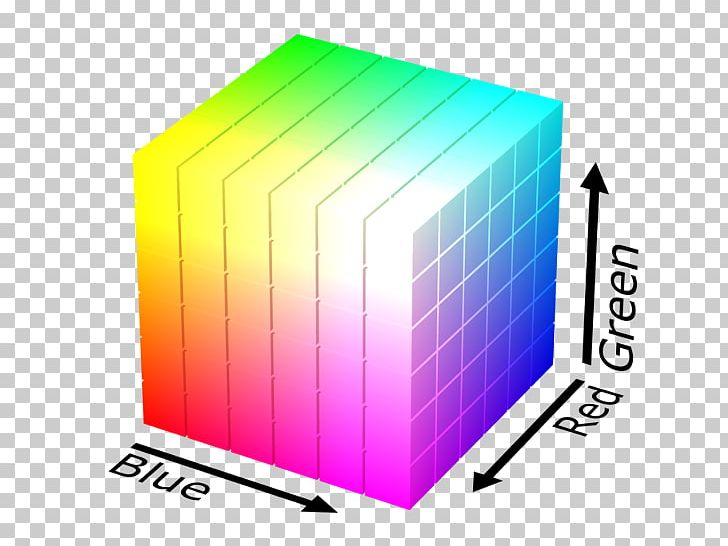
\includegraphics[width=5cm]{RGB_cube.jpg}\label{fig: RGB_cube}}
    \qquad
     \subfloat[][\centering HSV cone]{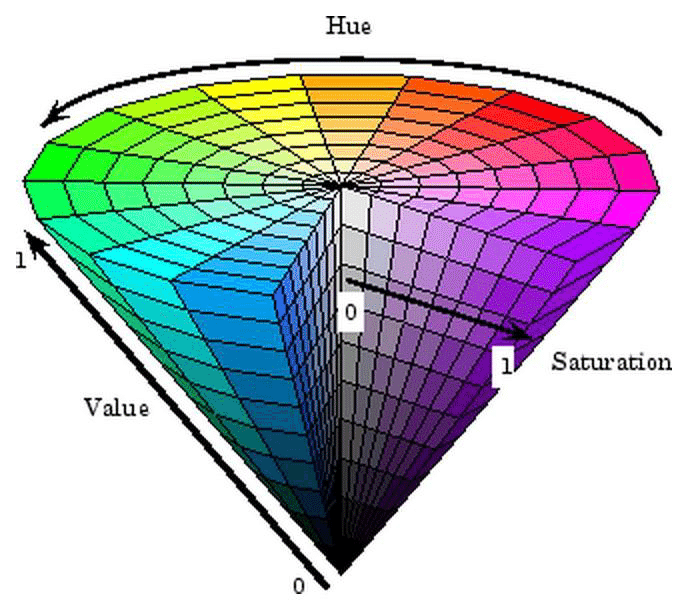
\includegraphics[width=5cm]{HSV_cone.png}\label{fig:HSV_cone}}
     \caption{Examples of color spaces}
     \label{fig:color_spaces}
\end{figure}

There are a lot of possible scales for representation\footnote{Besides RGB and CMYK \ref{fig: RGB_cube} the most common color spaces are CIE (Commision Internationale d’Eclairage) and HSV fig:\ref{fig:HSV_cone} (Hue,Saturation and Value). Refer to \cite{Color_spaces} for further details}, which are sometimes called color-spaces, however the most noteworthy in the scope of this work is the Hounsfield unit (HU) scale.

\begin{definition}[Hounsfield unit (HU)]
A scale used specifically to describe radiodensity, frequently used in the context of CT (Computed Tomography) exams. The values are obtained as a transformation of the linear attenuation coefficient \ref{eq:Lin_att_coef_def} of the material being imaged and, since the scale is supposed to be used on humans, it's defined such that water has value zero and air has the most negative value -1000. For  a more in depth discussion refer to \cite{Hounsfield}
\end{definition}

\begin{equation}\label{eq:HU_def}
    HU = 1000*\frac{\mu - \mu_{H_2O}}{\mu_{H_2O} - \mu_{Air}}
\end{equation}

The utility of this scale is in it's definition, since the pixel value depends on the attenuation coefficient it's possible to individuate a set of ranges that identify, within good reason, the various  tissues in the human body: for example lungs are [-700, -600] while bone can be in the [500, 1900] range.
A more in depth discussion of the topics relative to Hounsfield units is going to be carried out at a later point throughout this chapter, in the meantime it's necessary to clarify what are the most important characteristics of an image:

\begin{itemize}
\item Spatial Resolution: A measure of how many pixel are in the image or, equivalently, how small each pixel is; a larger resolution implies that smaller details can be seen better fig:\ref{fig:resolution_types}. Can be measured as the number of pixel measured over a distance of an inch ppi(Pixel Per Inch) or as number of line pairs that can be distinguished in a mm of image lp/mm (line pair per millimeter).
\item Gray-level Resolution: The range of the pixel values, a classic example is an 8-bit resolution which yields 256 levels of gray. A better resolution allows a better distinction of colors within the image fig:\ref{fig:resolution_types}.
    \todo[inline]{di solito si parla di color quantization}

\begin{figure}[H]
  		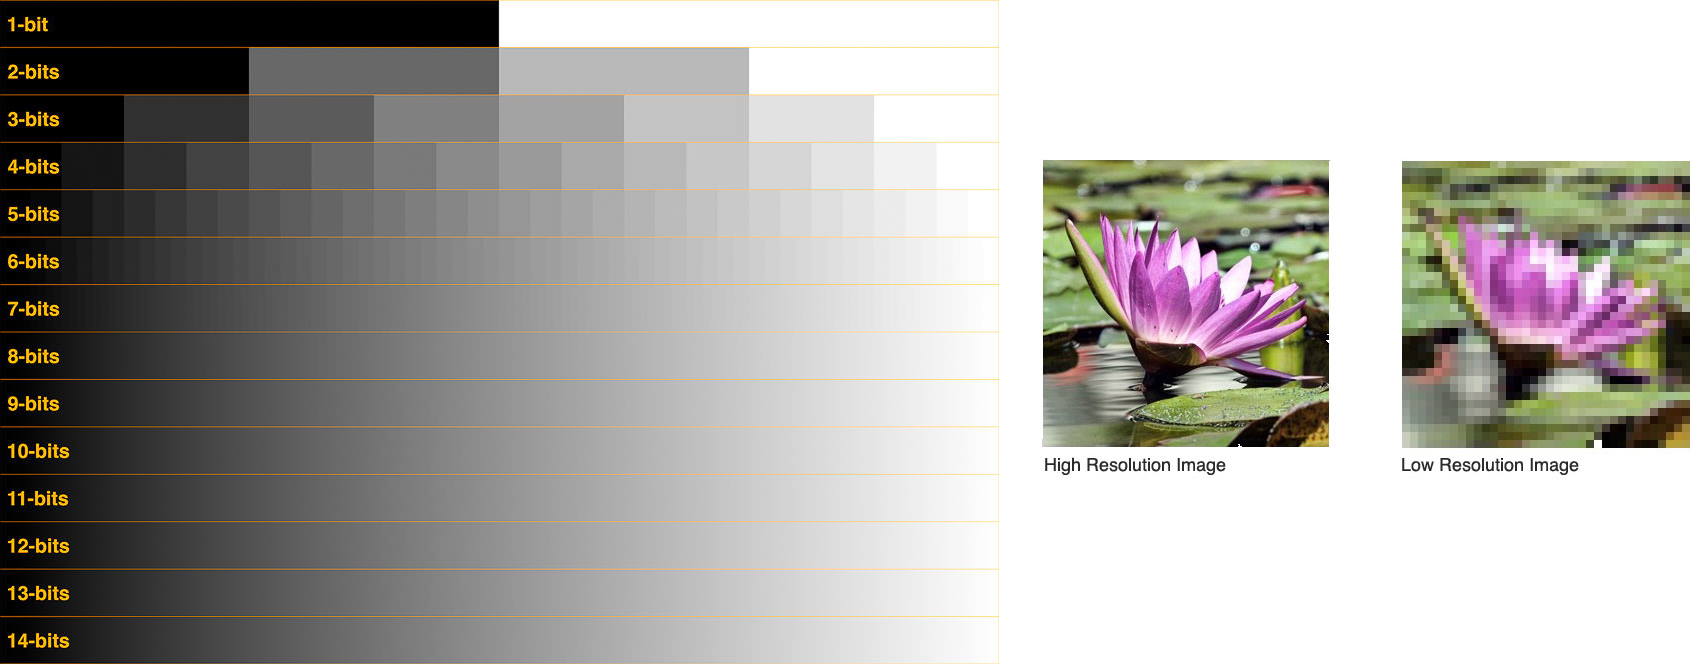
\includegraphics[width=0.8\textwidth]{Img_resolution.png}
        \caption{Example of visual differences in Gray-level (left) and spatial (right) resolution \label{fig:resolution_types}}
\end{figure}

\item Size: Refers to the number of pixel per side of the image, for example in CT-derived images the coronal slices are usually 512x512. These numbers depend on the acquisition process and instrument but in all cases these refer to the number of rows and columns in the sampling grid as well as in the matrix representing the image.
\item Data-Format: How the pixel values are stored in the file of the image. The most commonly used formats are .PNG and .JPG however there are a lot of other formats. In the context of this work, which is going to be centered on medical images, the most interesting formats are going to be the nii.gz (Nifti) and the .dcm (DICOM). The first contains only the pixel value information hence it's a lighter format, it originates in the field of Neuroimaging\footnote{In fact Nifti stands for Neuroimaging Informatics Technology Initiative (NIfTI)}, it is used mainly in Magnetic resonance images of the brain but also for CT scans and, since it contains only  numeric information, it's the less memory consuming option out of the two. The second contains not only the image data but also some data on the patient, such as name and age, and details on how the exam was carried out, such as machine used and specifics of the acquisition routine. This format is heavier than the previous one and, for privacy purposes, is much more delicate to handle which is why anonymization of the data needs to be taken in consideration. For a thorough description of the DICOM standard refer to \cite{DICOM}.
\end{itemize}

The format in which the image is saved depends on the compression algorithm used to store the information within the file. These algorithms can be lossy, in which case some of the information is lost to reduce the memory needed for storage, or lossless which means that all the information is kept at the expense of memory space. The first set of methods is preferred for storage of natural images, these are cases in which details have no importance, whereas the second set of methods is used where minute details can make a considerable difference such as in the medical field\footnote{A detailed description of compression algorithms is beyond the scopes of this thesis, for this reason please refer to \cite{Img_Compression} for more information}.

Given this set of characteristics it should now be clear that images can be thought of as array of numbers, for this reason they are often treated as matrices and, as such, there is a well defined set of valid operations and transformations that can be performed on them. All these operations and transformations, in a digital context\footnote{As opposed to analog context, which would mean the chemical processes used at the start of photography to develop and modify the film on which the image was stored}, are performed via computer algorithms which allow almost perfect repeatability and massive range of possible operations.

Given the list-like nature of images one of the most natural things to do with the pixel values is to build an histogram to evaluate some of the characteristic values of their distribution, such as average, min/max, skewness, entropy\ldots. The histogram of the image, albeit not being an unambiguous way to describe images, is very informative. When looking at an histogram it's immediately evident whether the image is well exposed and if the whole range of values available is being used optimally.

\begin{figure}[H]
  		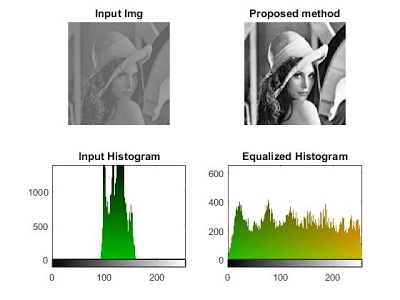
\includegraphics[width=0.8\textwidth]{Contrast_enhancement.jpg}
        \caption{Example of differences in contrast due to histogram equalization\label{fig:contrast_enhancement}}
\end{figure}

This leads us to the concept of \textit{Contrast} which is a quantification of how well different intensities can be distinguished. If all the pixel values are bundled in a small range leaving most of the histogram empty then it's difficult to pick up the differences because they are small however, if the histogram has no preferentially populated ranges then the differences in values are being showed in the best possible way fig:$\ref{fig:contrast_enhancement}$. Note also that if looking at the histogram there are two(or more) well separated distributions it's possible that these also identify different objects in the image, which will for example allow for some basic background-foreground distinction.

Assuming they are being meaningfully used \footnote{For example adding/subtracting one image to/from another can be reasonably understood, multiplying/dividing are less obvious but still used e.g. in scaling/mask imposition and change detection respectively} all mathematical operations doable on matrices can be performed on images for this reason it would be useless to list them all. However, it's useful to provide a list of categories in which transformations can be subdivided:

\begin{enumerate}
\item Geometric Transformations involve the following steps:
		\begin{enumerate}
		\item Affine transformations: Transformations that can can be performed via matrix multiplication such as rotations, scaling, reflections and translations. This step basically involves computing where each original pixel will fall in the transformed image
		\item Interpolation: Since the coordinates of the transformed pixel might not fall exactly on the grid it might become necessary to compute a kind of average contribution of the pixel around the destination coordinate to find a most believable value. Examples of such methods are linear, nearest neighbour and bicubic.
		\end{enumerate}
\item Gray-level (GL) Transformations: Involve operating on the value stored within the pixel, these can be further subdivided as:
		\begin{enumerate}
		\item Point-wise: The output value at specific coordinates depends only on the output value at those same specific coordinates. Some examples are window-level operations, thresholding, negatives and non-linear operations such as gamma correction which is used in display correction. Taken p as input pixel value and q as output and given a number $\gamma \in \mathbb{R}$, gamma corrections are defined as:
		\begin{equation}
		q = p^{\gamma}
		\end{equation}
    \item Local: The output value at specific coordinates depends on a combination of the original values in a neighbourhood around that same coordinates. Some examples are all filtering operation such as edge enhancement, dilation and erosion. These filtering methods are based on performing convolutions in which the output value at each pixel is given bu the sum of pixel-wise multiplication between the starting matrix and a smaller (usually 3x3 or 5x5) matrix called kernel. The output image is obtained by moving the kernel along the starting matrix following a predefined stride for example a (2,2) stride will move the kernel 2 pixels to the right and 2 down.
When moving near the borders the behavour is defined by the padding of the image, most common choice for padding is zero padding, in which the image is considered to have only zeros outside of it, or no padding at all. 
Stride \textbf{S}, kernel shape \textbf{K}
\footnote{This formula works for square kernels, images and strides so a kernel MxM will have K=M.}
 and padding \textbf{P} determine the shape of the output matrix given the input dimension \textbf{W} via the following formula:

\begin{equation}
Output Shape =\left[ \frac{W - K + P}{S}\right]+1
\end{equation}

		\item Global: The output value at specific coordinates depends on all the values of the original images. Most notable operation in this category is the Discrete Fourier Transform and it's inverse which allow switching between spatial and frequency domains. It's worth noting that high frequency encode patterns that change on small scales whereas low frequencies encode regions of the image that are constant or slowly varying.
		\end{enumerate}
\end{enumerate}

The aforementioned is surely not a comprehensive list of all that can be said on images however it should be enough for the scopes of this work.

\vspace{7mm} %7mm vertical space

Having seen what constitutes and image and what can be done with one it becomes interesting to explore how images are obtained. The following discussion is going to introduce briefly some of the methods used to obtain medical images, getting more in depth only on the modality used to obtain all the images used in this thesis which is Computed Tomography.
This technique was used because it's the only one that can provide information on the internal structure of an organ which is very low in density and that has parts that are deep in the patients body. Since no metabolic process of interest is in play PET is not advisable, Ultra Sounds are used for superficial soft tissue which is not the case of the lungs and MRI, despite it's clear advantege in avoiding ionizing radioation, still has close to no acquisition protocol dedicated to lungs.
\todo[inline]{perché hai scelto queste specifiche tecniche? a random?  Spiegato così va bene?}

\begin{enumerate}
\item Magnetic Resonance Imaging (MRI): This technique is based on the phenomenon of Nuclear Magnetic Resonance(NMR) which is what happens when diamagnetic atoms are placed inside a very strong uniform magnetic field are subject to Radio Frequency (RF) stimulus. These atoms absorb and re-emit the RF and supposing this behaviour can somehow be encoded with a positional dependence then it's possible to locate the resonant atoms given the response frequency measured. Suffices to say that this encoding is possible however the setup is very complex and the possible images obtainable with this method are very different and can emphasize very different tissue/material properties. Nothing more will be said on the topic since no data obtained with this methodology will be used. More details can be found in \cite{MRI}
\item Ultra-Sound (US): The images are obtained by sending waves of frequency higher to those audible by humans and recording how they reflect back. This technique is used mainly in imaging soft peripheral tissues and the contrast between tissues is given by their different responses to sound and how they generate echo. The main advantages such as low cost, portability and harmlessness come at the expense of explorable depth, viewable tissues, need for a skilled professional and dependence on patient bodily composition as well as cooperation.
\item Positron Emission Tomography (PET): In this case the images are obtained thanks to the phenomenon of annihilation of particle-antiparticle, specifically of electron-positron pairs.	The positrons come from the $\beta ^+$ decay of a radio-nucleide bound to a macromolecule, which is preferentially absorbed by the site of interest \footnote{Most commonly Fluoro-DeoxyGlucose FDG which is a glucose molecule labelled with a $^{18}$F atom responsible of the $\beta ^+$ decay. In general these radio-pharmaceuticals are obtained with particle accelerators near, or inside, the hospital that uses them. They are characterized by the activity measured as decay/s $\doteqdot$ Bq (read Becquerel) and half-life $\doteqdot$ T$_{\frac{1}{2}}$ which is how long it takes for half of the active atoms to decay}. Once the annihilation happens a pair of (almost) co-linear photons having (almost) the same energy of 511 keV is emitted, the detection of this pair is what allows the reconstruction of the image representing the pharmaceutical distribution within the body. Once again there are a lot of subtleties that are beyond the scopes of this thesis, suffices to say that: firstly the exam is primarily used in oncology given the greater energy consumption, hence nutrients absorption, of cancerous tissue and secondly this technique can be combined with CT scans to obtain a more detailed representation of the internal environment of the patient
\end{enumerate}

The last technique that is going to be mentioned is Computed Tomography however, given it's relevance inside this thesis work, it seems appropriate to describe it in a dedicated section.

\subsection{X-ray imaging and Computed Tomography (CT)}
It's well known that the term x-rays is used to characterize a family electromagnetic radiation defined by their high energy and penetrative properties. Radiation of this kind is created in various processes such as characteristic emission of atoms, also referred to as x-ray fluorescence, and Bremsstrahlung, braking radiation\footnote{From the German terms \textit{Bremsen} "to brake" and \textit{Strahlung} "radiation"}. The discovery that "A new kind of ray"\cite{Roentgen} with such properties existed was carried out by W.C.Roentgen in 1895, which allowed him to win the first Nobel prize in physics in the same year. Clearly the first imaging techniques that involved this radiation were much simpler than their modern counterpart, first of all they were planar and analog in nature, as well as not as refined in image quality. The first CT image was obtained in 1968 in Atkinson Morley's Hospital in Wimbledon. Tomography indicates a set of techniques\footnote{from the greek $\textit{Tomo}$ which means "to cut" and suffix -graphy to denote that it's a technique to produce images} that originate as an advancement of planar x-ray imaging; these techniques share most of the physical principles with planar imaging while overcoming some of it's major limitations, main of which being the lack of depth information.  X-ray imaging, both planar and tomographic, involves seeing how a beam of photons changes after traversing a target, the process amounts to a kind of average of all the effects occurred over the whole depth travelled.

The way in which slices are obtained is called focal plane tomography and, as the name suggests, the basic idea is to focus in the image only the desired depth leaving the unwanted regions out of focus. This selective focusing can be obtained either by taking geometrical precautions while using analog detectors, such as screen-film cassettes, or by feeding the digital images to reconstruction algorithms to perform digitally the required operations\footnote{In the first case the process is referred to as \textit{Geometric Tomography} while in the second case as \textit{Digital Tomosynthesis}}.

In both planar and tomographic setting the rough description of the data acquisition process can be summarized as follows: First x-rays are somehow generated by the machine, the quality of these x-rays is optimized with the use of filters then focused and positioned such that they mostly hit the region that needs imaging. The beam then exits the machine and starts interacting with the imaged object\footnote{In this work it's always going to be a patient, however this process is general and is also used in industry to investigate object construction}, this process causes an attenuation in the beam which depends on the materials composing the object itself. Having then travelled across the whole object it interacts with a sensor, be it film, semiconductor or other, which stores the data that will then constitute the final image. In a digital setting this final step has to be performed following a (tomographic) reconstruction algorithm which given a set of 2D projections returns a single 3D image.

In this light the interesting processes are how the radiation is created and shaped before hitting the patient and how said radiation then interacts with the matter of both the patient's body and the sensor beyond it. To explore these topics it's necessary to see:

\begin{itemize}
\item How these x-ray imaging machines are structured
\item How x-ray and matter interact as the first traverses the second
\end{itemize}

For more information on reconstruction algorithms refer to \cite{xray_reconstruction} and \cite{PhysicsMedicalImaging}.

\subsection{Generation and management of radiation: digital CT scanners}

As of the writing of this thesis, seven generations of CT scanners with different technologies used. The conceptual structure of the machines is mostly the same, and the differences between generations also make evident those between machines. Exploiting this fact the structural description is going to be only one followed by a brief list of notable differences between generations.

\begin{figure}[H]
\centering
  		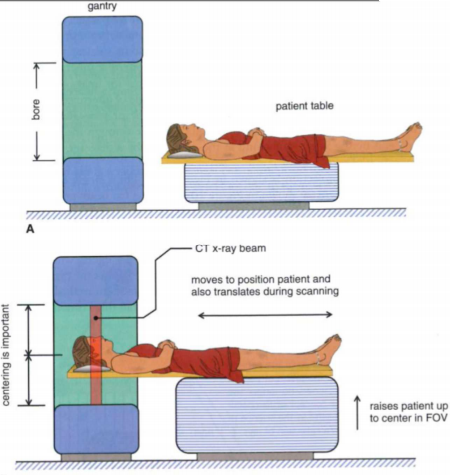
\includegraphics[scale=0.5]{CT_general.png}
        \caption{General set-up of a CT machine\label{fig:CT-machine}}
\end{figure}

The beam is generally created by the interaction of high energy particles with some kind of material, so that the particle's kinetic energy can be converted into radiation. In practice this means that an x-ray tube is encapsulated in the machine. Inside this vacuum tube charged particles\footnote{Most commonly electrons} are emitted from the cathode, accelerated by a voltage differential and shot onto a solid anode\footnote{Typical materials can be Tungsten, Molybdenum}. This creation process implies that the spectrum of the produced x-rays is composed of the almost discrete peaks of characteristic emission, due to the atoms composing the target, superimposed with the continuum Bremsstrahlung radiation.

\begin{figure}[H]
		\centering
  		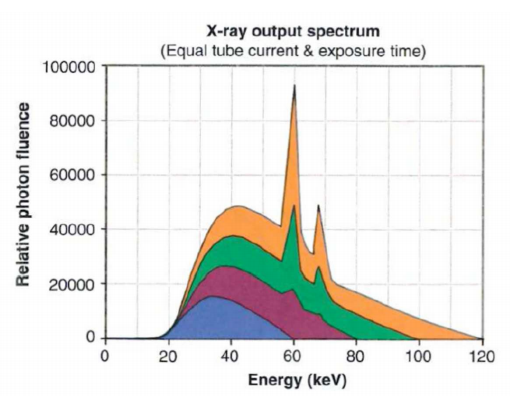
\includegraphics[width=0.8\textwidth]{xray_spectrum.png}
        \caption{X-ray spectrum, composed of characteristic peaks and Bremsstrahlung	continuum, computed at various tube voltages\label{fig:x-ray spectrum}}
\end{figure}

Some of the main characteristics of the x-ray beam are related to this stage in the generation, the Energy of the beam is due to the accelerating voltage in the tube  whereas the photon flux is determined by the electron current in the tube. Worth noting, en passant, that these two quantities can be found in the DICOM image of the exam as \textit{kiloVolt Peak (kVP)} and \textit{Tube current mA} and can be used to compute the dose delivered to the patient.

Other relevant characteristics in the tube are the anode material, which changes the peaks in the x-ray spectrum and time duration of the emission, which is called exposure time and influences dose as well as exposure\footnote{Exposure is a term used to identify how much light has gotten in the imaging sensor. Too high an exposure usually means the image is burnt, i.e. too bright and white, while lower exposures are usually associated to darker images. Exposure is proportional to the product of tube current and exposure time, measured in mA*s. Generally the machine handles the planning of exposure time according to treatment plan}.

The electron energy is largely wasted ($\sim 99\%$) as heat in the anode, which then clearly needs to be refrigerated. The remaining energy, as said before, is converted into an x-ray beam which is directed onto the patient. To reduce damage delivered to the tissues it's important that most of the unnecessary photons are removed from the beam.

Exploiting the phenomenon of beam hardening a filter, usually of the same material as the anode, is interposed between the beam and the patient to block lower energy photons from passing through thereby reducing the dose conveyed to the patient. At this point there may also be some form of collimation system which allows further shaping of the dose delivered. Having been collimated the beam traverses the patient and gets to the sensor of the machine, which nowadays are usually solid-state detectors.

At this point is where the differences between generations arise which, loosely speaking, can be found in the emission-detection configuration and technology.

\begin{itemize}
\item $1^{st}$ generation-Pencil Beam: A single beam is shot onto a single sensor, both sensor and beam are translated across the body of the patient and then rotated of some angle. The process is repeated for various angles. Main advantages are scattering rejection and no need for relative calibration, main disadvantage is time of the exam
\item $2^{nd}$ generation-fan Beam: Following the same process as the previous generation the main advantage is the reduction of the time of acquisition by introducing N beam and N sensors which don't wholly cover the patient's body so still need to translate.

\begin{minipage}{\linewidth}
            \centering
            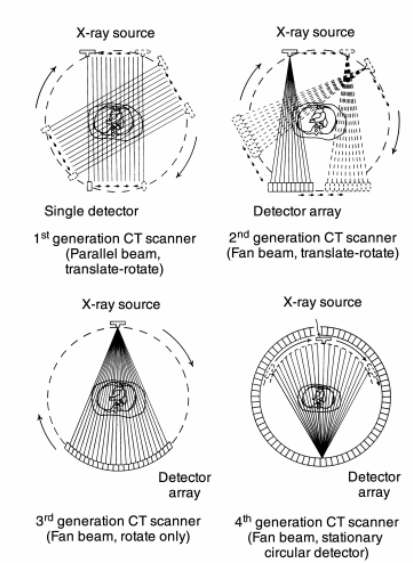
\includegraphics[width=6cm]{CT_gen1.png}
            \captionof{figure}{First four generation of CT scanners}
        \end{minipage}

\item $3^{rd}$ generation-Rotate Rotate Geometry: Enlarging the span of the fan of beams and using a curved array of sensor a single emission of the N beams engulfs the whole body so the only motion necessary is rotation of the couple beam-sensor array around the patient.
\item $4^{th}$ generation-Rotate Stationary Geometry: The sensors are now built to completely be around the patient so that only the beam generator has to rotate around the body \newline
\item $5^{th}$ generation-Stationary Stationary Geometry: The x-ray tube is now a large circle that is completely around the patient. This is only used in cardiac tomography and as such will not be described further \cite{Cardiac-CT}
\item $6^{th}$ generation-Spiral CT: Supposing the patient is laying parallel to the axis of rotation, all previous generations acquired, along the height of the patient, a single slice at a time. In this generation as the tube rotates around the patients the bed on which they're laying moves along the rotation axis so that the acquisition is continuous and not start-and-stop. This further reduces the acquisition time while significantly complicating the mathematical aspect of the reconstruction. It's necessary to add another important parameter which is the pitch of the detector\footnote{Once again the important parameters, such as this, can be accessed in the DICOM file resulting from the exam,}. This quantifies how much the bed moves along the axis at each turn the tube makes around the patient. Pitches smaller than one indicate oversampling at the cost of longer acquisition times, pitches greater than one indicate shorter acquisition times at the expense of a sparser depth resolution. \newline
\begin{minipage}{\linewidth}
            \centering
            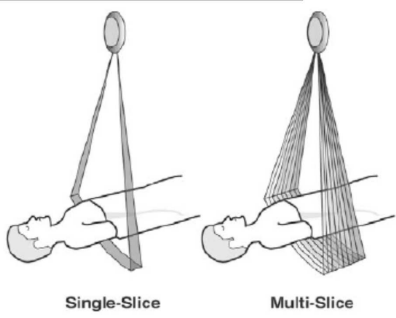
\includegraphics[width=6cm]{CT_gen2.png}
            \captionof{figure}{$7^{th} generation setup$}
        \end{minipage}
\item $7^{th}$ generation-MultiSlice: Up to this seventh generation height-wise slice acquisition was of a singular plane, be it continuous or in a start and stop motion. In this final generation mutliple slices are acquired. Considering cilindrical coordinates with z along the axis of the machine the multiple slice acquisition is obtained by pairing a fanning out along $\theta$ and one along z of both sensor arrays and beam. This technique returns to a start and stop technology in which only $\sim 50\%$ of the total scan time is used for acquisition
\begin{minipage}{\linewidth}
            \centering
            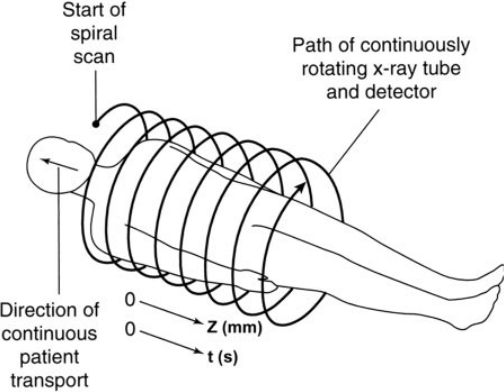
\includegraphics[width=6cm]{CT_gen3.png}
            \captionof{figure}{$7^{th} generation setup$}
        \end{minipage}
\end{itemize}

The machines used to obtain the images used in this thesis, all belonging to the Ospedale S. Orsola, were distributed as follows shown in \ref{fig:ct_dist}:


\begin{figure}[H]
\centering
  		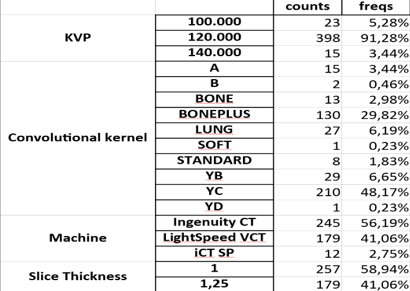
\includegraphics[]{CT_machines_distribution_fin.png}
        \caption{Acquisition parameter and machine distribution. KVP indicates the KiloVoltPeak used during the acquisition, Convolutional kernels are used by the factories to indicate which reconstruction algorithm is used. Machine indicated the name of the instrument that provided the images and slice thickness indicates the vertical width of the pixel.\label{fig:ct_dist}\todo[inline]{questa tabella richiede più dettagli di spiegazione. che cosa sono i numeri inseriti? la tabella dovrebbe poter essere compresa in modo completo senza troppi riferimenti al testo.}}
\end{figure}

\begin{enumerate}
\item Ingenuity CT  (Philips Medical Systems Cleveland):  $\sim 56\%$ of the exams were obtained with this machine
\item Lightspeed VCT  (General Electric Healthcare, Chicago-Illinois): $\sim 41\%$ of the exams in study come from this machine
\item ICT SP (Philips Medical Systems Cleveland):  $\sim 3\%$ of the exams were performed with this machine
\end{enumerate}

\subsection{Radiation-matter interaction: Attenuation in body and measurement}
Having seen the apparatus for data collection the remaining task is to see how the information regarding the body composition can be actually conveyed by photons.

Let's first consider how a monochromatic beam of x-rays would interact with an object while passing through it. All materials can be characterized by a quantity called attenuation coefficient $\mu$ which quantifies how waves are attenuated traversing them, this energy dependent quantity is used in the Beer-Lambert law which allows computation of the surviving number of photons, given their starting number $N_0$ and $\mu$:

\begin{equation}
N(x) = N_0e^{-\mu(E)*x}
\label{Beer-Lambert}
\end{equation}

At a microscopic level the absorption coefficient will depend on the probability that a photon of a given energy E interacts with a single atom of material. This can be expressed using atomic cross section $\sigma$ as:

\begin{equation}\label{Lin_att_coef_def}
\mu(E) = \frac{\rho*N_A}{A}*(\sigma_{Photoelectric}(E)+\sigma_{Compton}(E)+\sigma_{PairProduction}(E))
\end{equation}

Where $\rho$ is material density, $N_A$ is Avogadro's number, A is the atomic weight in grams and the distinction among the various possible interaction processes for a generic photon of high energy E is made explicit. Overall the behaviour of the cross section is the following

\begin{figure}[H]
\centering
  		\includegraphics[]{cross_section.png}
        \caption{Photon cross-section in Pb\label{fig:Photon-Cross-sect}}
\end{figure}

Overall, given eq:\ref{Beer-Lambert}, it's clear to see that the attenuation behaviour of a monochromatic beam would be linear in semi-logarithmic scale hence the name for $\mu$ "\textit{Linear Attenuation Coefficient}". The first complication comes from the fact that, given their generation method, the x-rays are not monochromatic but rather polychromatic. This introduces a further complication which is the phenomenon of beam hardening: lower energy x-rays interact much more likely than those at higher energies which implies that as it crosses some material the mean energy of the whole beam increases. This behaviour is exploited still within the machine, filters are interposed between anode and patient to reduce the useless part of the spectrum as shown in fig: \ref{fig:Beam-filtering}:

\begin{figure}[H]
\centering
  		\subfloat[Beam Filtering]{
  		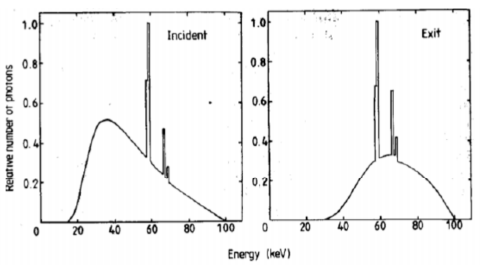
\includegraphics[scale=0.5]{Beam_Filtering.png}
        \label{fig:Beam-filtering}}
        \subfloat[Polychromatic beam attenuation]{
  		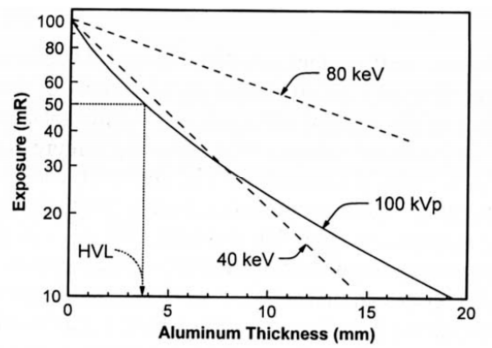
\includegraphics[scale=0.4]{Nonlin_attenuation.png}
        \label{fig:non_lin_attenuation}}
        \caption{Polychromatic beam behaviour}\label{fig:polychrom_behaviour}
\end{figure}

Another effect of the beam being polychromatic is that the graphical behaviour of the attenuation instead of being linear gets bent as shown in fig: \ref{fig:non_lin_attenuation}. Since the image brightness is related to the number of photons that get on the sensor it's still possible to define the contrast between two pixel $p_1, p_2$ as:

\begin{equation}
C(p_1,p_2) = \frac{N_{\gamma ,p_2}-N_{\gamma ,p_1}}{N_{\gamma ,p_2}}
\end{equation}

This formula, that connects the beam to the image, together with eq: \ref{Beer-Lambert}, which connects the beam property to the patient's composition, make clear the processes by which the beam carries patient information. Another complication arises in the context of this last equation due to the phenomenon of scattering which reduces the contrast by changing the direction of the bean and introducing an element of noise. Anti-scattering grids are positioned right before the sensors to reduce this effect by allowing to reach the sensor to only the photons with the correct direction.

The biological effects of radiation won't be treated in this thesis. Suffices to say that damage can be classified as primary, due to ionization events within the nucleus of the cell, or secondary, due to chemical changes in the cell environment. The energy deposited per unit mass is called dose and is measured in Gy(Gray) and, as said before, depends on exposure time, current and kVP of the tube. Most of contemporary machines for CT self-regulate exposure time during the acquisition automatically using Automatic Exposure Control(AEC). Having the dose it's possible to estimate the fraction of surviving cells and, to do so, various models are used. In the clinical practice it's common to find, still within the DICOM image metadata, the information regarding Dose delivered such as CTDI (Computed Tomography Dose Index) from which it's possible to obtain the DLP (Dose Length Product) taking into consideration the total length of irradiated body. For an introduction to one of these models, the Linear Quadratic (LQ) refer to \cite{LQ_model}.\newline

\section{Artificial Intelligence (AI) and Machine Learning(ML)}
Having clarified the type of data that will be used in this work, and having seen the general procedure used to gather it, it becomes interesting to discuss what kind of techniques will be used to analyze it.

Starting from the definition given by John McCarthy in \cite{AI_def} "[AI] is the science and engineering of making intelligent machines, especially intelligent computer programs. It is related to the similar task of using computers to understand human intelligence, but AI does not have to confine itself to methods that are biologically observable.". Machine Learning (ML) is a sub-branch of AI and contains all techniques that make the computer improve performances via experience in the form of exposure to data, practically speaking this finds it's application in classification problems, image/speech/pattern recognition, clustering, autoencoding and others. The general workflow of Machine Learning is the following: given a dataset, the objective is to define a model or function  which depends on some parameters which is able to manipulate the data in order to obtain as output something that can be evaluated via a predefined performance metric. The parameters of the model are then automatically adjusted in steps to minimize or maximize this performance metric until a stable point at which the model with the current parameters is considered finalized; one of the main problems in this procedure is being sure that the stable point found is global and not local. The whole procedure is carried out keeping in mind that the resulting model needs to be able to generalize it's performance on data that it has never seen before, for this reason usually ML is divided in a training phase and a testing phase. The training phase involves looking at the data and improving the performance of the model on a specific dataset\footnote{Usually in studies there is a single dataset which is split into a train-set and a test-set, in some cases if the model is good it can be validated prospectively, which means that it's performance is evaluated on data that did not yet exist at the time of birth of the model}, the testing phase involves using brand new data to evaluate the performance of the model obtained in the preceding phase. Machine Learning techniques can be further grouped into the following categories:

\begin{enumerate}
\item Supervised Learning: In this type of ML the model is provided with the input data as well as the correct expected output, which is hence called \textit{label}. The objective of the model is to obtain an output as similar to the labels as possible, while also retaining the best possible generalization ability in predicting never seen before data. Some problems that benefit from the use of these techniques are regression and classification problems.
\item Unsupervised Learning: As the name suggests this category of models trains on the data alone, without having the labels available by minimizing some metric defined from the data. For example clustering techniques try to find a set of groups in the data such that the difference within each group is minimal while the difference among groups is maximal, ideally producing dense groups, called clusters, that are each well separated from all the others. Other techniques in this family are Principal Component Analysis (PCA) and autoencoding but the general objective is to infer some kind of structure within the data and the relation between data points.
\item Reinforcement Learning:  This kind of ML is well suited for data which has a clear sequential structure in which the requiered task is to develop good long term planning. Broadly speaking the general set-up is that given a set of (state$_{t}$, action, reward, state$_{t+1}$) these techniques try to maximize the cumulative reward\footnote{i.e. the sum of the rewards obtained at all previous time steps}. The main applications of these techniques are in Autonomous driving and learning how to play games
\end{enumerate}

The following methods are those directly involved in this work.

\subsection{Regression, Classification and Penalization}
Regression and Classification are methods used to make predictions via supervised learning by understanding the input-output relation in continuous and discrete cases respectively. The most basic example of regression is linear regression which consists in finding the slope and intercept of a line passing through a set of points. A branch of classification thats similar to linear regression is logistic regression, this translates in finding out wether or not each point belongs to a certain category given it's properties and can be practically thought of, for a binary classification,as a fitting procedure such that the output can be either 0 for one category and 1 for the other, this is usually done using the logistic funtion, also called sigmoid, which compresses $\mathbb {R}$ in [0,L] as seen in  \ref{sigmoid}. L represents the maximum value desidered, $x_0$ is the midpoint and k is the steepness. Note that for multiple categories it would conceptually suffice to add sigmoids with different centers to obtain a step function in which each step corresponds to a category, in this case the procedure is usually called multinomial regression.
\begin{equation}
\sigma_{(x)} = \frac{L}{1+e^{-k(x-x_0)}}
\end{equation}

\begin{figure}[H]
		\centering
  		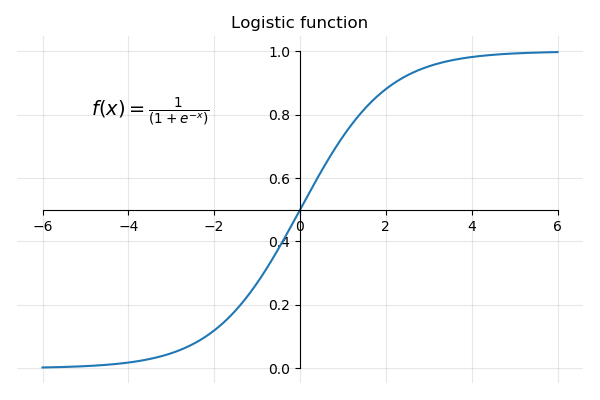
\includegraphics[width=0.8\textwidth]{Sigma_curve.png}
        \caption{sigmoid function with L=1, $x_0$=0, k=1 \label{sigmoid}}
\end{figure}

To give a general intuition of the procedure, without going in unnecessary details, let's only consider linear regression; the theory on which it is founded is based on the assumption that the residuals, i.e. the distance model-label, are normally distributed. Under this assumption the parameters can be found by changing them and trying to minimize the sum of squared residuals.

When each datapoint is characterized by a lot of different features the procedure is called multiple linear regression, the task becomes finding out how much each feature contributes in predicting the output within a weighted linear combinaion of features. Practically speaking this can be done in matricial form, supposing that each of the m datapoints has n features associated let  \textbf{X} be a matrix with n+1\footnote{n+1 because we have n features but we also want to estimate the intercept of the line, so in practice the first column will be of all ones to have the correct model shape in the following matrix multiplication} columns and m rows and let  \textbf{Y} be a vector with m entries. Let also  \textbf{$\theta$} be a vector of n+1 entries, one for each feature plus the intercept $\theta_0$, then we are supposing that:

\begin{equation}
y_i = \Sigma^{n+1}_{j=0} x_{i,j}*\theta_i + \epsilon_i =>  \textbf{Y} =  \textbf{$X*\theta$} + \textbf{$\epsilon$}
\end{equation}

Where $\epsilon$ is the array of residuals of the model which, as said before, is supposed to contain values that are normally distributed. Minimizing the squared residuals corresponds to minimizing the following cost function:

\begin{equation}
J_{\theta} =   (\textbf{Y} - \textbf{$X*\theta$})^T*(\textbf{Y} - \textbf{$X*\theta$})
\end{equation}

By setting $\frac{\delta J}{\delta \theta}$=0 it can be shown that the best parameters \textbf{$\theta^*$} are :

\begin{equation}
\textbf{$\theta^*$}=    (\textbf{X}^T* \textbf{X})^{-1}*\textbf{X}^T\textbf{Y}
\end{equation}

It's evident that to obtain a result from the previous operation it's necessary that $(\textbf{X}^T* \textbf{X})$ be invertible, which in turn requires that there be no correlated features and that the features be less than the datapoints. To solve this problem  the first step is being careful in choosing the data that goes through the regression, which may even involve some preprocessing. The second step is called Regularization,  it involves adding a penalty to the cost function by adding a small quantity along the diagonal of the matrix. The nature of this small quantity changes the properties of the regularization procedure, the most famous penalties are Lasso, Ridge and ElasticNet.  In practical terms the shape of the penalty determines how much and how fast the slopes relative to the features can be shrunk.

\begin{enumerate}
\item Ridge: Adds $\delta^2 * \Sigma^{n+1}_{j=1} \theta_j^2$, is called also $L^2$ regularization since it adds the $L^2$ norm of the parameter vector. This penalty can only shrink parameters asymptotically to zero but never  exactly, which means that all features will always be used,  even with very small contributions
\item Lasso: Adds $\frac{1}{b} * \Sigma^{n+1}_{j=1} |\theta_j|$, is called also $L^1$ regularization since it adds the $L^1$ norm of the parameter vector. This penalty can shrink parameters to exactly zero, getting rid of the useless variables within the model.
\item ElasticNet: Adds $\lambda*[\frac{1-\alpha}{2}  * \Sigma^{n+1}_{j=1} \theta_j^2$ + $\alpha* \Sigma^{n+1}_{j=1} |\theta_j|]$, evidently this is a midway between  the Lasso and Ridge methods, where the balance is dictated by the value of $\alpha$.
\end{enumerate}
\todo[inline]{visto che usi la regolarizzazione in modo consistente spiegherei meglio i vantaggi dei vari approcci uno rispetto all'altro}

Following regularization procedures, specifically Lasso regularization, as a byproduct of avoiding divergences a selection and ranking of the important features is obtained however it's still important to preprocess the data to simplify the job of the regularization.

Since the whole foundation is the normality of the residuals it's important that the data behaves somewhat nicely in this regard. Changing the data to modify the residuals is not straightforward, a proxy for this procedure is to preprocess the data by manipulating the distribution of the features to make them as close to normal as possible.
To this end some of the operations that can be done are:

\begin{enumerate}
\item Standard Scaling: This amounts to subtracting the mean of the distribution to the feature and dividing by the standard deviation so that the resulting distribution is somewhat centered around zero and has close to unitary standard deviation
\item  Boxcox transform: When distributions are heavy-tailed, like a gamma distribution would be, this finds the best exponent to transform via a power-law the data. Since the exponent $\lambda \in$$\mathbb{R}$ the input data needs to be strictly positive and not constant.\todo[inline]{la spiegherei meglio}
\end{enumerate}

Practical application of these procedures can be found in  cap:\ref{cap: Material_method}. These considerations conclude the theoretical background on regression, classification and penalization thereof.

\subsection{Decision Trees and Random Forest}
Apart from logistic and multinomial regression there are various other supervised classifiying methods such as Support Vector Machines (SVM), Neural Networks and Decision Trees. In this thesis, among the aforementioned algorithms, the chosen one was a particular evolution of DecisionTrees called RandomForest (RF).
To provide some insight in the method it's necessary to first explain how decision trees work, specifying what problems they face and what are their strong points.
Since it's a classification method let's consider the simple case of binary classification with categorical\footnote{Categorical is to be intended as features with discrete value, opposed to continuous variables which can potentially take any value in $\mathbb{R}$} features. The task of the decision tree is to approximate to the best of it's abilities the labels contained in the training set using all the features associated with each datapoint, this is done by building a graph-like structure in which the nodes represent the features and the links departing from it are the possible values the feature takes. This graph is built in a top-down approach by choosing at every step the feature that best separates the data in the label categories, this process is done along each branch unitl a node in which the separation of the preceding feature is better then that provided by all remaining features or all features have been considered. The first node is called root node, while the nodes that have no branches going out of them are called leaves, the graph represents a tree hence the name of the method. Note that at every node only the subset of data corresponding to all previous feature categories is used.
At each node the separation between the two label categories $c_1, c_2$ due to the feature is commonly measured with Gini impurity coefficient, which is computed as:

\begin{equation}
	\begin{split}
		G &= 1 - p^2_1 -p^2_2 \\
		   &= 1 - \left[ \frac{N_{c_1\in node}}{N_{samples\in node} } \right]^2 - \left[\frac{N_{c_2\in node}}{N_{samples\in node}} \right]^2
	\end{split}
\end{equation}

The Gini impurity for a feature is then computed as an average of the gini coefficients of all the deriving nodes weighted by the number of samples in each of the nodes.  This method can be obviously generalized to cases in which features are continuous by thresholding the features choosing the value that best improves the separation of the deriving node, a way to choose possible thresholds is to take all the means computed with all adjacent measurements. It's important to note firstly that there is no restiction on using, along different branches, different tresholds for the same feature and, secondly, that the same featue can end up at different depths along diffenrent branches. The strength of this method is it's performance on data it has seen however it has very poor generalization abilities \cite{StatisticalLearning}. 

Random Forests algorithms are born to overcome this problem. As the name suggests the idea is to build an ensemble of Decision Trees in which the features used in the nodes are chosen among random subsamples of all the available features, the final result is obtained as a majority vote over all trained trees. Each tree is also trained on a bootstapped dataset created from the original, this procedure might exacerbate some problems of the starting dataset by changing the relative frequency of classes seen by each tree and can be corrected by balancing the bootstrap procedure.

This method vastly improves the performance and robustness of the final prediction while retaining the simplicity and ease of interpretation of the decision trees, naturally there are methods, such as AdaBoost, to deploy and precautions, such as having balanced dataset, to take to further improve the performance of RF classifiers.

In the context of this thesis it will become necessary to take care of balancing the input dataset, to do so one could randomly oversample, by duplicating instances in the minority class, or undersample, by removing instances within the majority class. The choice that was made was to use Synthetic Minority Oversampling TEchnique (SMOTE)\cite{SMOTE} to rebalance the dataset.

\subsection{Synthetic Minority Oversampling TEchnique (SMOTE)}
This technique considers a user-defined number of nearest neighbours of randomly chosen points in the minority class and populates the feature space by generating samples on the lines that connect the chosen sample with a random neighbour\footnote{This procedure is formally called convex combination, which is a peculiar linear combination of vector in which the coefficients sum to one. Particularly all convex combination of two points lay on the line that connects them, and for three point lay within the triangle that has them as vertices}.


\begin{figure}[H]
		\centering
  		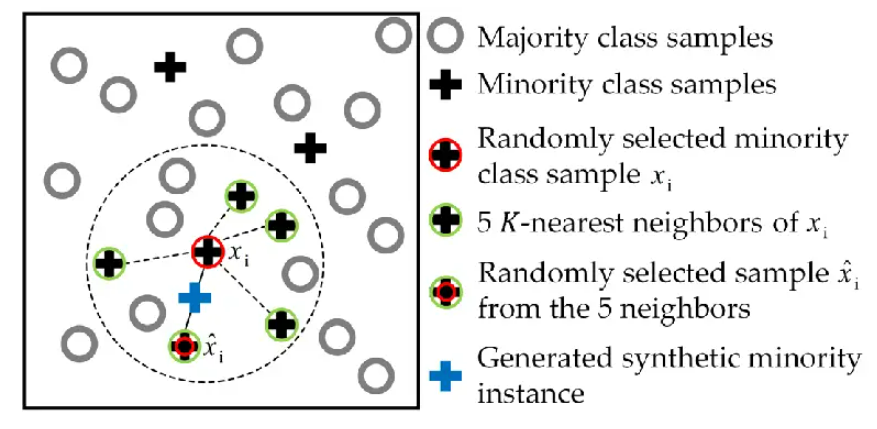
\includegraphics[width=0.8\textwidth]{SMOTE.png}
        \caption{Example of SMOTE with 5 nearest neighbours}
\end{figure}

Worth noting that this has been done using the library imblearn in python \cite{imblearn}. To preview some of the data, looking at the performance of a vanilla random forest implementation with all preset parameters, the effect of the position of oversamplling is the following.


\begin{figure}[H]
\centering
  	\subfloat[][without smote]{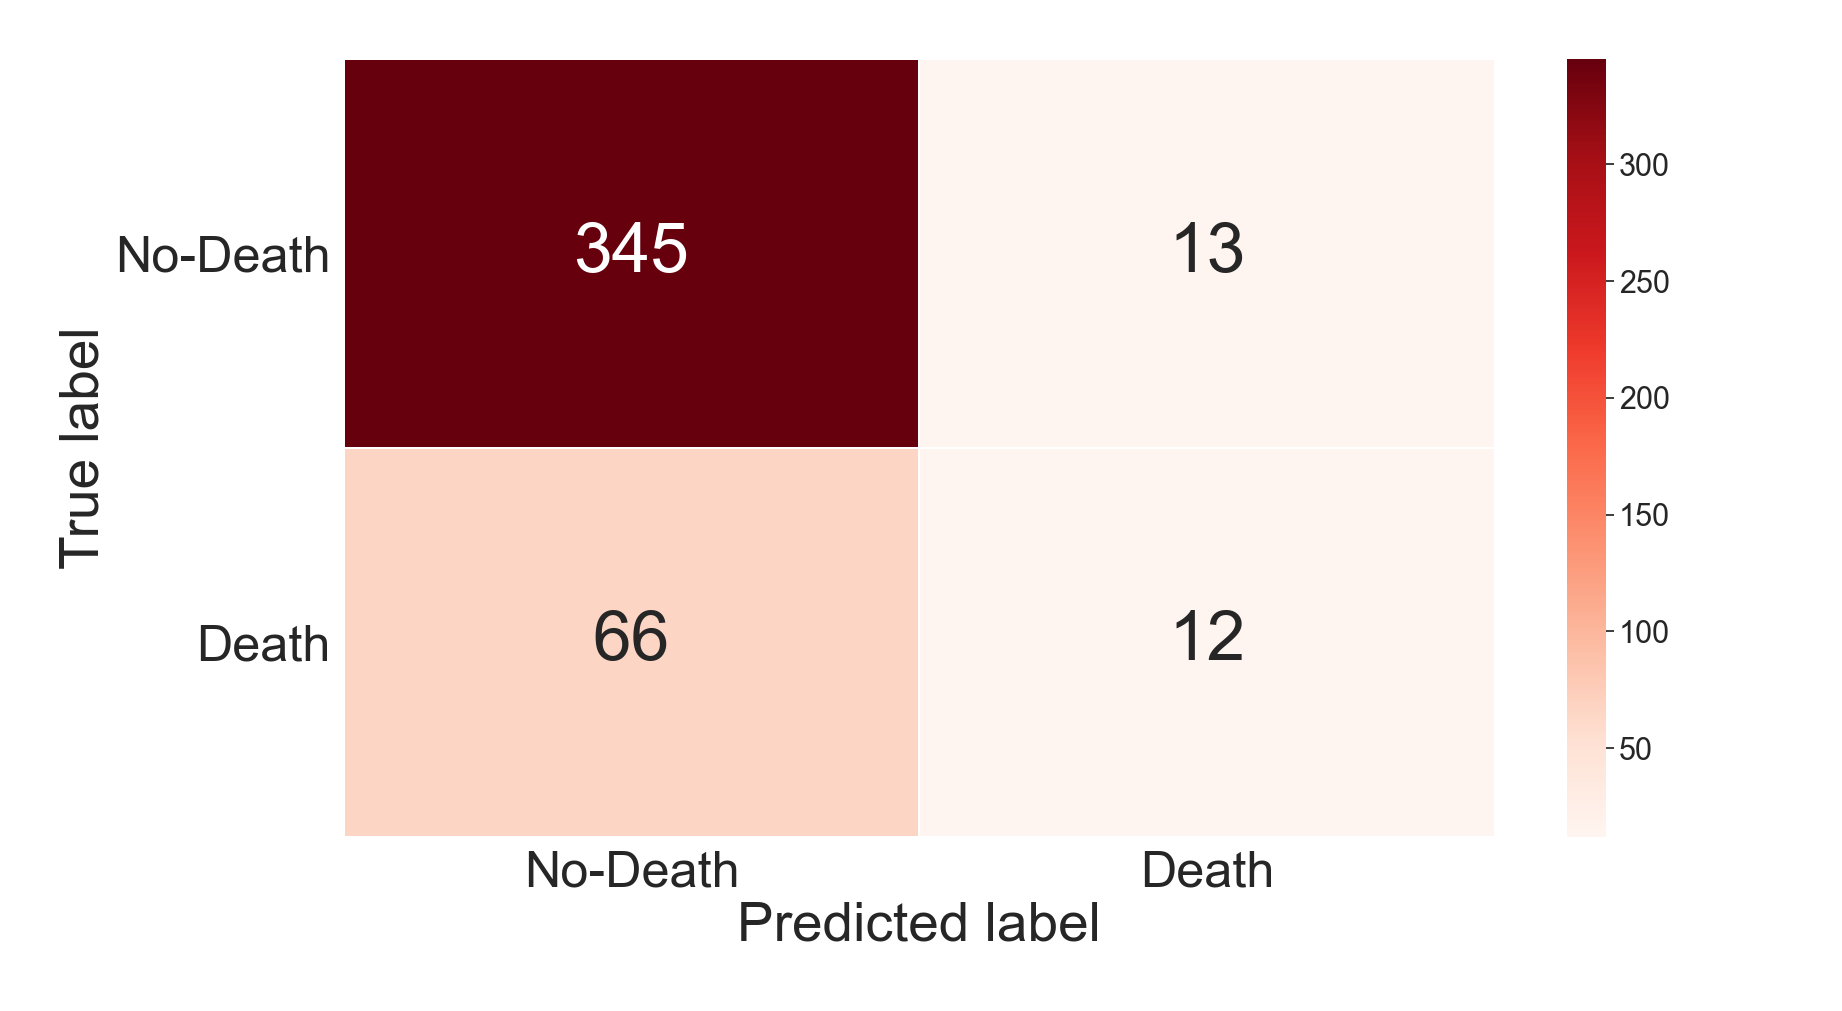
\includegraphics[width=0.50\linewidth]{RF_Death.png}\label{fig:smoteless}}
        \subfloat[][SMOTE-before train-test split]{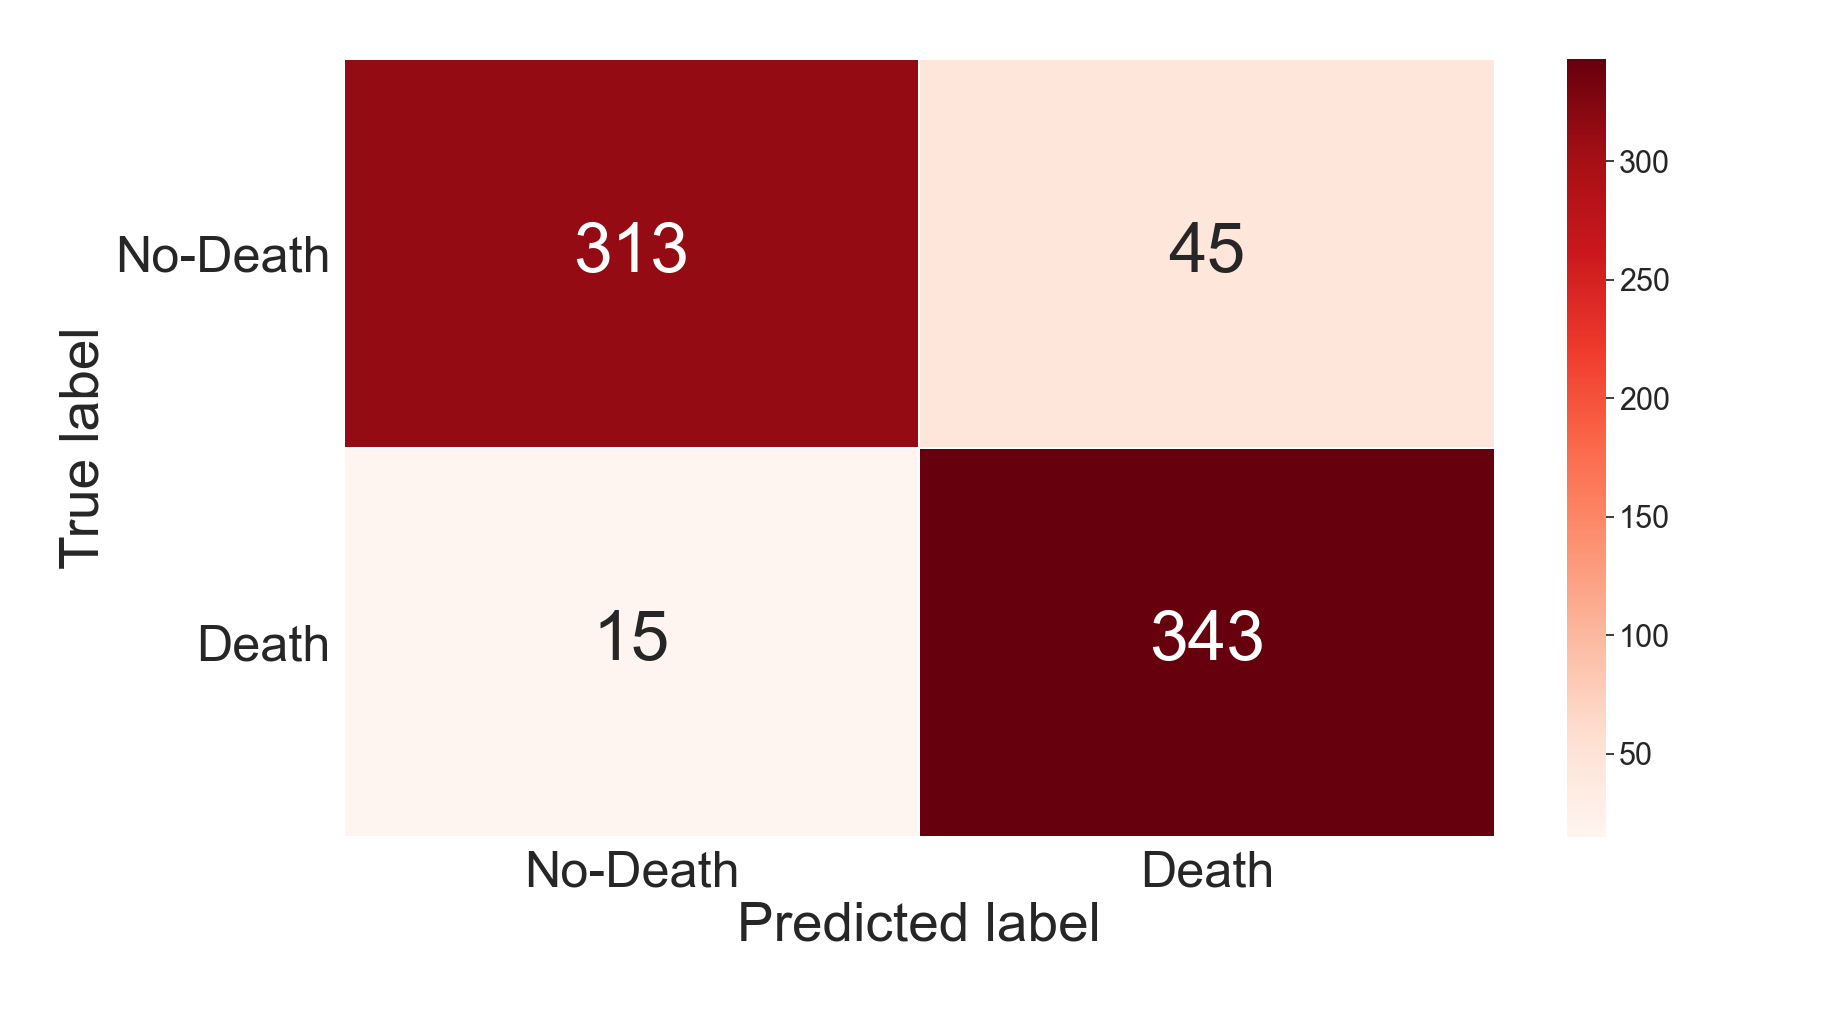
\includegraphics[width=0.503\linewidth]{RF_Smote_Death.png}\label{fig:smote_before}}
\centering \newline
	\subfloat[SMOTE after train-test split]{\includegraphics[width=0.50\linewidth]{Death_Smote.png}\label{fig:smote_after}}
    \caption{Confusion matrix used to evaluate performance done using datasets with various combinations of SMOTE position \todo[inline]{queste figure devono avere i numeri ed il testo più grandi, sono illeggibili altrimenti; inoltre i risultati delle divisioni vanno inseriti dopo, non qui.} }\label{fig:smote_after}
\end{figure}

It's clear to see that in unbalanced case, like the one analysed in this thesis in which the label classes are 15$\%$-85$\%$, oversampling the data always determines an improvement in performance. However performing it in the wrong place it clearly makes a far too optimistic evaluation of the performance. This highlights the point that all preprocessing should be done with care when train-test splitting the data, specifically it's very important that the oversampling, as well as all other data handling, be performed after the train-test split of the data on the train data alone. It's clear to see that what's being observed is a leakage phenomenon, in which the testing data contiains information regarding the training data and viceversa. In practice, especially because the points are created as convex combination of existing data\footnote{Note that this would happen with any other over/under-sampling methods, such as random oversampling which randomly duplicates data points}, when the synthetically generated points end up in the testing they depend, at least partially, on the data used in the training procedure.

\subsection{Dimensionality reduction and clustering}
When dataset are composed of many features, namely more than three, it becomes difficult if not impossible to visualize the distribution of data. There are various techniques that can mitigate or solve this problem, they are grouped under the umbrella term of "Dimensionality reduction techniques" and they are generally based on ML learning methods. As such , following the same reasoning and definitions given in regard to ML, it's possible to introduce a sub-categorization of the whole family of techniques in supervised and unsupervised techniques. Dimensionality reduction, beyond providing useful insight in the general structure of the data, can also be used as a preprocessing step in some analysis pipelines. A first example could be to find more meaningful features before analyzing with methods such as Random Forests or Regression techniques, a second example could be using the reduced representation that keeps the most information possible to ease in clustering analysis by highlighting the differences in subgroups within the dataset. The most common dimensionality reduction techniques are:

\begin{enumerate}
\item \textbf{Unsupervised methods}
	\begin{itemize}
		\item Principal Component Analysis (PCA): Linearly combines the pre-existing features to obtain new ones and orders them by decreasing ability to explain total variance of data. The first principal component is the combination of features that most explains the variance in the original dataset. Given it's nature it focuses on the global characteristics of the dataset.
		\item t-distributed Stochastic Neighbor Embedding (t-SNE): Keeps a mixture of local and global information by using a distance metric in the full high dimensional space and trying to reproduce the distances measured in the lower dimensional space which can be 2- or 3-dimensional. {\large NON SO SE VA SPIEGATO MEGLIO O PIU' IN DETTAGLIO}\newline
			Let's define similarity between two points as the value taken by a normal distribution in a point away from the centre, corresponding to the first point of interest, the same distance as the two points taken in consideration. Fixing the first point the similarities with all other points can be computed and normalized. Doing this procedure for all points it's poissible to build a normalized similarity matrix. Then the whole dataset is projected in the desired space, usually $\mathbb{R}^i$ with i=1,2 or 3, in which a second similarity matrix is built using a t-distribution instead of a normal distribution \footnote{The use of this t-distribution gives the name to the technique, the need for this choice is to avoid all the points bunching up in the middle of the projection space since t-distributions have lower peaks and are more spread out than normal distributions. For more details refer to \cite{t-sne}}. At this point, in iterative manner, the points are moved in small steps in directions such that the second matrix becomes more similar to the one computed in the full space.
\end{itemize}

\item \textbf{Supervised methods}
	\begin{itemize}
	\item Partial Least Squared Discriminant Analysis (PLS-DA): This technique is the classification version of Partial Least Squares (PLS) regression. Much like PCA the idea is to find a set of orthonormal vectors as linear combination of the original features in the dataset, however in PLS and PLS-DA is necessary to add the constraint that the new component, besides being perpendicular to all previous ones, explains the most variability in a given target variable, or set thereof. For an in depth description refer to \cite{PLSDA} while for a more modern review refer to \cite{PLSDA_review} \large{Hanno senso queste due in bibliografia?}
	\end{itemize}

\item \textbf{Mixed techniques}
	\begin{itemize}
		\item Uniform Manifold Approximation and Projection (UMAP): Builds a network using a variable distance definition on the manifold on which the data is distributed then uses cross-entropy as a metric to reproduce a network with the same structure in the space with lower dimension. This technique maintains very local information on the data and allows a complete freedom in the choice of the final embedding space as well as the definition of distance metrics in the feature space\footnote{Actually to keep the speed in performance the distance function needs to be Numba-jet compilable}, it's also implemented to work an a generic pandas dataframe in python so it can take in input a vast range of datatypes. The math behind this method is much beyond the scopes of this thesis, as such refer to \cite{UMAP} for more in depth information.
	\end{itemize}
\end{enumerate}

It should be noted that dimensionality reduction is not to be taken as a necessary step, however it can reduce the noise in the data by extrapolating the most informative features while easing in visualization and reducing computational costs of subsequent data analysis. These upsides become particularly relevant in the field of clustering, where the objective is to group data in sets with similar features by minimizing the differences within each group while maximizing the differences between different groups. Clustering techniques can be roughly divided in:

\begin{enumerate}
\item Centroid based techniques: A user defined number of points is randomly located in the data space, datapoints are then assigned to groups according to their distance from the closest center. The main technique in this category is k-means clustering, and some, if not most, other techniques include it as step in the processing pipeline\footnote{An example of such techniques is: affinity propagation}. The main problems are firstly that these techniques require prior knowledge, or at the very least a good intuition, on the number of clusters in the dataset  while also assuming that the clusters are distributed in spherical gaussian distribution, which is not always the case.
\item Hierarchical clustering: The idea is to find the hierarchical structure in the data using a bottom-up or a top-down approach, as such this category further subdivides in agglomerative and divisive methods. In the first each point starts by itself and then points are agglomerated using a similarity or distance metric, this build a dendrogram in which the k$^{th}$ level roughly corresponds to a k-centrouid clustering. In the latter the idea is to start with a unique category and then divide it in subgroups.
\item Density based techniques: These methods use data density to define the groups by looking for regions with larger and lower density as clusters and separations.
\end{enumerate}

In order to evaluate the performance of these methods it's necessary to define metrics that evaluate uniformity within clusters and separation among them, the choice in the definition of metric should be taken in careful consideration since the different task may imply very different optimal metrics or, put differently, the optimal technique for the task at hand may very well depend on the metric used.

It's worth mentioning that when working in two, or at most three, dimensions humans are generally good at preforming clustering yet it's nearly impossible to do in more dimensions. Computers, on the other hand, require more careful planning even in low dimension but are much more performing even in higher dimensions because the generally good human intuition on the definition of cluster is not so easily translated in instruction to a machine. So to obtain good results with clustering techniques it necessary to work with care, expecially with a good understanding of the dataset in use and it's overall structure.

In the context of this thesis, supposing the data suggested a clear cut distinction of two populations in the dataset, as could be male-females or under- vs  normal- vs over-weight individuals, then it might become necessary to analyse these groups as different  cohorts in order to more accurately predict their clinical outcome.


\section{Combining radiological images  with AI: Image segmentation and Radiomics}
Having seen the kind of data that will be of interest throughout this thesis, and having a set of techniques used describe and make predicition on the data at hand, the final step in this theoretical background chapter will be to combine these two notion in describing first how images can be treated in general terms and then, more specifically, how medical images can be analysed to exploit as much as possible the vast range of information they contain.

Image analysis seems, at first glance, very intuitive since for humans it's very easy to infer qualitative information from images. However upon closer inspection this matter becomes clearly non trivial due to the subjectivity involved in the process as well as in the intuition behind it. More specifically, in the context of this thesis, the same image of damaged lungs contains very different informations to the eyes of trained professional versus those of an ordinary person as well as to the eyes of different professionals.

The first big obstacle in this task is the definition of region of interest: not all people will see the same boundary in a damaged organ, sometimes the process of defining a boundary between organ and tissue may need to account for the final objective it has to achieve. If the objective is to evaluate texture of a damaged lung then the lesion needs to be included whereas in other cases these regions may only be unwanted noise. Generally speaking finding regions of interest in an image is a process called image segmmentation.

The next step would be to quantify the characteristics of the region identified, as such it should be clear that finding ways to derive objective information from images it's of paramount importance, expecially when this information can aid in describing the health of a patient. It should also be clear that medical images are a kind of high dimensional data as such, as it's fashion with fields that occpy themselves with big biological data, the field that studies driving quantitative information out of radiological images is called radiomics.

\subsection{Image Segmentation}
Generally speaking image segmentation is a procedure in which an image is divided in smaller sets of pixels, such that all pixel inside a certain set have some common property and such that there are no overlaps between sets. These sets can then be used for further analysis which could mean foreground-backgroud distinction, edge detection as well as object detection, computer vision and pattern recognition. Image segmentation can be classified as:

\begin{itemize}
\item Manual segmentation: The regions of interest are manually defined usually by a trained individual. The main advantage of this it's the versatility, on the other hand this process can be very time consuming
\item Semi-automatic segmentation: A machine defines as best as it can the shape of the region of interest, however the process is then thought to receive intervention of an expert to correct the eventual mistakes or refine the necessary details. This provides the best compromise between time needed and accuracy obtained and becomes of interest in fields in which finer details are important.
\item Automatic segmentation: A machine performs the whole segmentation without requiring human intervention
\end{itemize}

On a practical level these techniques can be used in various fields, as illustrated by the variety of aforementioned tasks, but the one that interests this work the most is the medical field.
Nowadays in medicine, where most of imaging exams are stored in digital form, the ability to automatically discern specific structures within the images can provide a way to aid clinical professionals in their everyday decision making their workload lighter and helping in otherwise difficult cases.
A staggering example connected to this thesis is the process of organ segmentation in CT scans: usually these scans are n\footnote{n clearly depends on the exam required and slice thickness, some common values for thoracic CTs are around 200-300 but can range up to 900 slices} stacked images in 512x512 resolution. To have a contour of the lungs in a chest CT a radiologist would need to draw by hand the contour of the lung in each slice of the scan. Even if some shorcuts exist to reduce the number of slices to draw on this very boring, time consuming and repetitive task can occupy hours if not days of work to a human  while a machine can take minutes to complete a whole scan. Then considering lesion detection in medical exams having a machine that consistently finds lesions that would otherwise be difficult to discern by a human eye can be of paramount importance in diagnosis as well as treatment.
In the medical field the difficulty comes from the fact that different exams have different types of image formats which means that an algorithm that works well on CT may not work as intended on MRI or other procedures.
Automatic image segmentation can be performed in various ways:

\begin{enumerate}
\item Artificial Neural Network (ANN): These techniques belong to a sub-field in ML called Deep Learning, they involve building network structures with more layers in which each node is a processing unit that takes a combination of the input data and gives an output according to a certain activation function. These structures are called Neural Networks because they resemble and are modeled after the workings of neuron-dendrite structures while the deep in deep learning refers to the fact that various layers composed of various neurons are stacked one after the other to complete the structure. Learning is obtained by changing how each neuron combines the inputs it recieves. In the case of images these structures are called Convolutional Neural Networks because the first layers, which are intended to extract the latent features or structures in the images, perform convolution operation in which the parameters are the values pixel values of convolutional kernels
\item Thresholding: These techinques involve using the histogram of the image to identify two or more groups of pixel values that correspond to specific parts/objects within the image. An obvious case would be a bi-modal distribution in which the two sets can be clearly identified but there are no requirements on the histogram shape.  In the case of CT this has a very simple and clear interpretation since HU depend on tissue type it's reasonable to expect that some tissues can be differentiated with good approximation by pixel value alone
\item Deformable models and Region Growing: Both these technique involve setting a starting seed within the image, in the first case the seed is a closed surface which is deformed by forces bound to the region of interest, such as the desired edge. In the second case the seed is a single point within the region of interest, step by step more points are added to a set which started as the seed alone according to a similarity rule  or a predefined criteria.
\item Atlas-guided: By collecting and summarizing the properties of the object that needs to be segmented it's possible to compare the image at hand with these properties to identify the object within the image itself.
\item Classifiers: These are supervised methods that focus on classifying via by focusing on a feature space of the image. A feature space can be obtained by applying a function to the image, an example of feature space could be the histogram. The main distinction from other methods is the supervised approach
\item Custering: Having a starting set of random clusters the procedure computes the centroids of these clusters, assigns each point to the closest cluster and recomputes centroids. This is done iteratively until either the point distribution or the centroid position doesn't change significantly between iterations.
\end{enumerate}

 For a more in depth review of the main methods used in medical image segmentation refer to \cite{Medical_img_segmentation}. Worth noting, at this point, that the semi-automatic segmentation software used in this work uses probably a mixture of region growing and thresholding methods, maybe guided by an atlas.
The segmentation process generally produces a boolean mask which can be used to select, using pixel-wise multiplication, the region of interest in the image. The next step in image analysis would be to derive information from the region defined during segmentation, in general this step is called feature extraction\footnote{Even if the term is used in pattern recognition as well as machine learning in general} and it's objective is to find non-redundant quantities that meaningfully summarize as much properties of the original data as possible.

\subsection{Radiomics}
 When the images are medical in nature and when referring to high-throughput quantitative analysis the task of finding these features fall in the realm of radiomics, which uses mathematical tools to describe properties of the images that would otherwise be unquantifiable to the human eye. The features that can be computed from images are of various types, some of them can be understood somewhat easily through intuition since they are close to what humans generally use to describe images, others are much more complex in definition and quantify more difficulty percieved properties of the image. Features can be then roughly classified in different families:

\begin{enumerate}
\item Morphological features: These features describe only the shape of the region of interest, as such they are independent of the pixel values inside the region and hence, to be computed, require only a boolean mask of the segmented region. These features can be further subcategorized as two or three dimensional features based on whether they focus on single slices or whole volumes. Most of these features compute volumes, lengths, surfaces and shape properties such as sphericity, compactness, flatness and so on.
\item First order features: These features depend strictly on the gray levels within the region of interest since they evaluate the distribution of these values, as such they need that the boolean mask of the segmentation be multiplied pixel-wise with the origian image to obtain a new image with only the interesting part in it. Most of these features are commonly used quantities, such as Energy, Entropy, Minimum and Maximum value which have been adapted to the imaging context using the histogram of the original image or by considering intensities within an enclosed region.
\item Higher order features: All the other fatures fall in this macro-category which can be clearly subdivided in other smaller catgories in which the features are obtained following the same guiding principle or starting point. Generally these describe more texture-like properties of the image and, to do so, use particular matrices derived from the original image which contain specific information regarding order and relationships in pixel value positioning within the image. These matrices have very precise definition, as such only the general idea behind them will be reported here redirecting to \cite{IBSI} for a more strict and in detail description. The matrices from which the features are computed also give name to the smaller categories in this family, these categories are:
	\begin{itemize}
		\item Gray Level Co-occurence Matrix (GLCM) features: This matrix expresses how combination of pixel values are distributed in a 2D or 3D region by considering connected all neighbouring pixel in a certain direction with respects to the one in consideration. Using all possible directions for a set distance, usually $\delta$=1 or $\delta$=2, various matrices are obtained and from these a probability distribution can be built and evaluated. It should be noted that before computing these matrices the intensities in the image are discretized.
		\item Gray Level Run Length Matrix (GLRLM) features: Much like before the task of these features is to quantify the distribution of relative values in gray levels trhoughout the image, as the name suggests what this matrix quantifies is how long a path can be built by connecting pixel of the same value along a single direction. This time information from the matrices computed by considering different directions are aggregated in different ways to improve rotational invariance of the final features
		\item Gray Level Size Zone Matrix (GLSZM) features: This matrix counts the number of zones in which voxel have the same discretized gray level. The zones are defined by a notion of connectedness most commonly first neighbouring voxel are considered as connectable if they have the same value, this leads to a 26 neighbouring voxel in 3 dimensions and to 8 connected pixels in 2 dimensions\footnote{To visualize, imagine a 2D grid: the 8 pixel are the four at the sides of each square and the four at the corners.}. The matrix contains in position (i,j) the number of zones of size j in which pixel have value i.
		\item Neighbouring Gray Tone Difference Matrix (NGTDM) features: Born as an alternative to GLCM these features rely on a matrix that contains the sum of differences between all pixel with a given pixel value and the average of the gray levels in a neighbourhood around  them.
		\item Gray Level Dependence Matrix (GLDM) features: The aim of these features is to capture in a rotationally invariant way the texture and coarsness of the image. This matrix requires the already seen concept of connectedness with a given distance as well as dependence among pixel. Two voxel in a neighbourhood are dependent if the absolute value of the difference between their discretized value is less then a certain threshold. The number of dependent voxel is then counted with a particular approach to guarantee that the value be at least one
	\end{itemize}
\end{enumerate}

In talking about the previous feature groups the concept of discretization of data which is already digital, and hence a discretized, has emerged. This is often a required step to make the computations of the matrices tractable and consists in further binning together the pixel values, which is commonly done in two main ways: either the number of bins is fixed or the width of the bins is fixed preceeding the discretization process.
It should be evident that the results of the feature extraction procedure is heavily dependent on the choices made in all the steps that preceed it, main of which being the segmentation, the eventual re-discretization of the image leading to the algorithm used to compute the feature themselves. For this reason recently the International Biomarker Standardization Initiative (IBSI \cite{IBSI}) wrote a \textit{"reference manual"} which details in depth the definitons of the features, description of data-processing procedures as well as a set of guidelines for reporting results. This was done in an attempt to reduce as much as possible the variability and lack of reproducibility of radiomic studies.
In the past the main attention in radiological research was focused on improving machine performances and evaluating acquisition sequence technologies, however the great developements in artificial intelligence and performance of computers have brought a lot of attention to the field. Various papers, such as \cite{Rad_review} and \cite{Rad_review_ger} have been written with the objective of presenting the general workflow. By design the topics in this thesis have been presented to resemble the general order of the pipeline, which can be summarised as:

\begin{itemize}
\item Data acquisition
\item Definition of the Region Of Interest (ROI)
\item Pre-processing
\item Feature extraction
\item Feature selection
\item Classification
\end{itemize}

Another interesting possibility offered by the biomarkers computed following radiomics is the ability to quatify the differences between successive exams of the same patient. This specific branch of radiomics is called Delta-radiomics, referencing to the time differential that become the main focus of the analysis.
{\large NON SAPREI SE VA BENE COSI' O BISOGNA AGGIUNGERE ALTRI DETTAGLI}

With this the theoretical background has been laid out and the thesis can finally proceed to practically and more specifically describing the data at hand as well as the specific techniques used to elaborate it.

\section{Survival Analysis}
Survival analysis is a particular field that tries to determine the probability of a certain event happening before a certain time.
As the name suggests one of it's main application is determining the risk of death due to a disease as time progresses from diagnosis, however it can be used to estimate time needed to recover after a surgical procedure, lifetime before breakdown of machines, time needed for criminals to commit new crimes after being released \ldots. 

The main concepts and terminologies in this field are:

\begin{enumerate}
\item Event: This is the phenomenon under analysis, generally it could be death, remission from recovery, recovery \ldots .
It is common to refer to the event as failure since usually the event is a negative event.
\item Censoring: When colelcting data to develop a model that describes survival it may happen that the individual drops out of the study without incurring in the event under analysis.
For example when looking at effectiveness of a drug the patient develops an adverse reaction to the drug and needs to stop using it, hence falling out of the study.

In the context of this thesis all individuals that got sent home from the hospital are censored since their survival is known only up until the dropout and not after.
Cases like this when the start of the followup is well known but dropout happens are called right-censored, because only the right side of the timeline is abruply interrupted.
Cases can also be left-censored, e.g. a patients with unknown time of contraction of a disease, and interval-censored, e.g. when the contraction of the disease can be restricted to an interval as it may happen when a negative and positive test happen at successive times.

Usually this variable is called \textbf{d} and is a binary variable where 1 indicates that the event occurred and 0 indicates all possible censoring causes.
\item Time: This is to be intended as time, be it days, weeks, months or years, since the start of the followup to either the event or the censoring.
It usually is indicated with \textbf{T}, is referred to as survival time and, being a random variable that indicates time, it cannot be negative.
\item Survivor function \textbf{S(t)}: This is to be intended as the probability that the subject in the study survives a time t before incurring in the event.
In theory this function is smooth from zero to infinity, it's strictly non-increasing, it starts at S(0)=1 and ends up at S($\infty$)=0.

These assumptions are all resonable since at no point the survival probability can increase, since everybody is alive at the start of observing them and since nobody can live to infinity.
However, when it comes to practice, these properties are not necessarily verified.
Since no study can continue to infinity the last value need not be zero and since the timesteps at which it's possible to perform a checkup are discrete the curve is actually a step function.
\item Hazard Function \textbf{h(t)}: This function is difficult to explain practically, citing \cite{SurvivalAnalysis} \textbf{"The hazard function h(t) gives the instantaneous potential per unit time for the event to occur, given that the individual has survived up to time t"}. The mathematical definition is:
\begin{equation}
h(t) = \lim\limits_{\Delta t \to 0} \frac{P(t\leq T < t + \Delta t | T\geq t)}{\Delta t}
\end{equation}
Dividing by a time interval the hazard function can also be intended as conditional failure rate, where the conditional refers to the "given that the individual has survived up to time t". Being a rate this quantity need not be bound in [0,1] but ranges in [0, $\infty$] and depends on the time unit used.
 This will be interpreted as h(t) events per unit time.

The hazard function is non-negative and has no upper bounds, since it can be related to the survival function
\footnote{The hazard function can be computed as time derivative of the survival function divided by the survival function changed of sign. The survival function is the exponential of minus the integral in [0,t] of the hazard function. On this note, an exponential model is given by a constant hazard function. loosely speaking the Weibulls and LogNomal respectively come from increasing, decreasing and somewhat bell-shaped hazard functions.} 
the possible shapes give different names to the final model. 
These could be increasing or decreasing Weibull, exponential or lognormal survival models
\end{enumerate}

A further step in the analysis could be to try to measure the differences in survival between two groups, i.e. using a single variable expected to drive the differences in survival.
The most basic example would be looking at the effectiveness of a drug by dividing in group A and B the patients given the actual medicine and the placebo respectively, however this could be done even for males vs females or, in the case of continuous variables, for patients with above or below threshold values
\footnote{Generally, when no obvious threshold is available, the median of the variable is chosen.}.
When the analysis is univariate in nature then the Kaplan-Meier survival curves are used in conjuction with the log-rank test, when the analysis is multivariate then the Cox Proportional-Hazard model is used. 
The Cox model is very similar to linear and logistic regression.

Explaining these methods is beyond the scopes of this thesis, all details can be found in \cite{SurvivalAnalysis}.
Suffices to say that, as rule of thumb, two Kaplan-Meier curves that do not intersect at any point indicate good separation among the groups which can then be evaluated using the p-value from the log-rank test.
When it comes to Cox models they can be used to create a new variable, much like the linear combination of variables in linear regression, which in turn can be used to identify groups in the patient cohort. This division in groups can be obtained using the median, or the percentiles if one desires more than two groups. 
The division in the resulting groups can be used as proxy for the quality of the score built using the Cox model.
